\documentclass[10pt]{article}\usepackage[]{graphicx}\usepackage[]{color}
%% maxwidth is the original width if it is less than linewidth
%% otherwise use linewidth (to make sure the graphics do not exceed the margin)
\makeatletter
\def\maxwidth{ %
  \ifdim\Gin@nat@width>\linewidth
    \linewidth
  \else
    \Gin@nat@width
  \fi
}
\makeatother

\definecolor{fgcolor}{rgb}{0.345, 0.345, 0.345}
\newcommand{\hlnum}[1]{\textcolor[rgb]{0.686,0.059,0.569}{#1}}%
\newcommand{\hlstr}[1]{\textcolor[rgb]{0.192,0.494,0.8}{#1}}%
\newcommand{\hlcom}[1]{\textcolor[rgb]{0.678,0.584,0.686}{\textit{#1}}}%
\newcommand{\hlopt}[1]{\textcolor[rgb]{0,0,0}{#1}}%
\newcommand{\hlstd}[1]{\textcolor[rgb]{0.345,0.345,0.345}{#1}}%
\newcommand{\hlkwa}[1]{\textcolor[rgb]{0.161,0.373,0.58}{\textbf{#1}}}%
\newcommand{\hlkwb}[1]{\textcolor[rgb]{0.69,0.353,0.396}{#1}}%
\newcommand{\hlkwc}[1]{\textcolor[rgb]{0.333,0.667,0.333}{#1}}%
\newcommand{\hlkwd}[1]{\textcolor[rgb]{0.737,0.353,0.396}{\textbf{#1}}}%

\usepackage{framed}
\makeatletter
\newenvironment{kframe}{%
 \def\at@end@of@kframe{}%
 \ifinner\ifhmode%
  \def\at@end@of@kframe{\end{minipage}}%
  \begin{minipage}{\columnwidth}%
 \fi\fi%
 \def\FrameCommand##1{\hskip\@totalleftmargin \hskip-\fboxsep
 \colorbox{shadecolor}{##1}\hskip-\fboxsep
     % There is no \\@totalrightmargin, so:
     \hskip-\linewidth \hskip-\@totalleftmargin \hskip\columnwidth}%
 \MakeFramed {\advance\hsize-\width
   \@totalleftmargin\z@ \linewidth\hsize
   \@setminipage}}%
 {\par\unskip\endMakeFramed%
 \at@end@of@kframe}
\makeatother

\definecolor{shadecolor}{rgb}{.97, .97, .97}
\definecolor{messagecolor}{rgb}{0, 0, 0}
\definecolor{warningcolor}{rgb}{1, 0, 1}
\definecolor{errorcolor}{rgb}{1, 0, 0}
\newenvironment{knitrout}{}{} % an empty environment to be redefined in TeX

\usepackage{alltt}
% !Rnw weave = knitr
%
%\makeatletter
%% \VignetteIndexEntry{An overview of psd.}
%% \VignetteEngine{knitr}
%\makeatother
%
\usepackage[T1]{fontenc}
\usepackage[utf8]{inputenc}
\usepackage{fancyvrb}
\usepackage[pdfborder={0 0 0}]{hyperref}
\usepackage{url}
\usepackage{upquote}
\usepackage{graphicx}
\usepackage{grffile}
\usepackage{float}
\usepackage{natbib}
\usepackage{amsmath}
\usepackage{hyperref}
\usepackage{geometry}
\geometry{verbose,tmargin=3cm,bmargin=5cm,lmargin=2.5cm,rmargin=2.5cm}
\usepackage[font=sf, labelfont={sf,bf}, margin=2cm]{caption}
\usepackage{color}
%
\newcommand{\SC}[1]{\textsc{#1}}
\newcommand{\SCY}[0]{\SC{Yes}}
\newcommand{\SCN}[0]{\SC{No}}
\newcommand{\Rcmd}[1]{\texttt{#1}}
\newcommand{\psd}[0]{\href{http://www.github.com/abarbour/psd/}{\color{blue}\Rcmd{psd}}}
%% path, filename, caption, label
\newcommand{\listing}[4]{        %
  \begin{figure}[H]              %
    \centering                   %
    \VerbatimInput[numbers=left, %
      frame=single,              %
      label=#2]{#1}              %
    \caption{#3}                 %
    \label{#4}                   %
  \end{figure}                   %
}
\author{Andrew J. Barbour and Robert L. Parker}
\title{An overview of \psd{}: Adaptive sine multitaper power spectral density estimation in R}
\IfFileExists{upquote.sty}{\usepackage{upquote}}{}
\begin{document}
\maketitle
\begin{abstract}
  This vignette provides an overview of some 
  features included in the package \psd{}, designed to
  compute estimates of power spectral
  density (PSD) for a univariate series in a sophisticated manner,
  with very little tuning effort.
  The sine multitapers are used, and
  the number of tapers varies with spectral shape, according
  to the optimal value proposed by \citet{rs1995}.
  The adaptive procedure
  iteratively refines the optimal number of tapers at each frequency
  based on the spectrum from the previous iteration.
  Assuming the adaptive procedure converges, 
  this produces power spectra
  with significantly
  lower spectral variance 
  relative to results from less-sophisticated estimators.
  Sine tapers exhibit excellent
  leakage suppression characteristics, so bias effects
  are also reduced.
  Resolution and uncertainty vary with the number of tapers,
  which means we do
  not need to resort to either (1) windowing methods,
  which inherently degrade resolution at low-frequency
  (e.g. Welch's method); or (2) smoothing kernels,
  which can badly distort important features without careful tuning
  (e.g. the Daniell kernel in \Rcmd{stats::spectrum}).
  In this regards
  \psd{} is best suited for data having 
   large dynamic range and some mix of narrow and wide-band structure,
   features typically found in geophysical datasets.
\end{abstract}

\tableofcontents
\pagebreak


%opts_knit$set(verbose = TRUE)

\section{Quick start: A minimal example.}
First, we load the package into the namespace:
%% libload
\begin{knitrout}
\definecolor{shadecolor}{rgb}{0.969, 0.969, 0.969}\color{fgcolor}\begin{kframe}
\begin{alltt}
\hlkwd{library}\hlstd{(psd)}
\end{alltt}


{\ttfamily\noindent\itshape\color{messagecolor}{\#\# Loading required package: fftw\\\#\# Loaded psd (0.5.0) -- Adaptive multitaper spectrum estimation}}\end{kframe}
\end{knitrout}
For a series to analyze, we can use \Rcmd{magnet}, included in \psd{},
which represents along-track measurements
of horizontal magnetic-field strength from a gimbaled, airborne magnetometer.
These data are a small subset of the full Project MAGNET series \citep{coleman1992},
which has provided insight into
the history of the Earth's oceanic crust 
\citep{parker1997, obrien1999, korte2002}.
The sampling interval is
once every kilometer (km), so the data will represent
crustal magnetization with wavelengths longer than 2 km.
%% Project MAGNET data
\begin{knitrout}
\definecolor{shadecolor}{rgb}{0.969, 0.969, 0.969}\color{fgcolor}\begin{kframe}
\begin{alltt}
\hlkwd{data}\hlstd{(magnet)}
\end{alltt}
\end{kframe}
\end{knitrout}
The format of the data set is a \Rcmd{data.frame} with four
sets of information:
%%
\begin{knitrout}
\definecolor{shadecolor}{rgb}{0.969, 0.969, 0.969}\color{fgcolor}\begin{kframe}
\begin{alltt}
\hlkwd{names}\hlstd{(magnet)}
\end{alltt}
\begin{verbatim}
## [1] "km"    "raw"   "clean" "mdiff"
\end{verbatim}
\end{kframe}
\end{knitrout}
The \Rcmd{raw} and \Rcmd{clean} names represent raw
and edited intensities respectively, expressed in units of nanotesla; 
\Rcmd{mdiff} is the difference between them.
The difference between them is a matter of just a few points
attributable to instrumental malfunction. 
%% edits
\begin{knitrout}
\definecolor{shadecolor}{rgb}{0.969, 0.969, 0.969}\color{fgcolor}\begin{kframe}
\begin{alltt}
\hlkwd{subset}\hlstd{(magnet,} \hlkwd{abs}\hlstd{(mdiff)}\hlopt{>}\hlnum{0}\hlstd{)}
\end{alltt}
\begin{verbatim}
##      km    raw   clean     mdiff
## 403 402  209.1 -3.6355 -212.7355
## 717 716 -248.7 -9.7775  238.9225
\end{verbatim}
\end{kframe}
\end{knitrout}
These deviations can,
as we will see, adversely affect the accuracy of any PSD estimate,
multitaper or otherwise.

We can find power spectral density (PSD)
estimates for the two series quite simply with \Rcmd{pspectrum}:
%% pspectrum 5 iters
\begin{knitrout}
\definecolor{shadecolor}{rgb}{0.969, 0.969, 0.969}\color{fgcolor}\begin{kframe}
\begin{alltt}
\hlstd{psdr} \hlkwb{<-} \hlkwd{pspectrum}\hlstd{(magnet}\hlopt{$}\hlstd{raw)}
\end{alltt}


{\ttfamily\noindent\itshape\color{messagecolor}{\#\# Stage\ \ 0 est. (pilot) \\\#\# 	environment\ \ ** .psdEnv **\ \ refreshed\\\#\# detrending (and demeaning)\\\#\# 1024 --> 1024}}

{\ttfamily\noindent\bfseries\color{errorcolor}{\#\# Error: min\_taper * max\_taper >= 1 \& max\_taper >= min\_taper is not TRUE}}\begin{alltt}
\hlstd{psdc} \hlkwb{<-} \hlkwd{pspectrum}\hlstd{(magnet}\hlopt{$}\hlstd{clean)}
\end{alltt}


{\ttfamily\noindent\itshape\color{messagecolor}{\#\# Stage\ \ 0 est. (pilot) \\\#\# 	environment\ \ ** .psdEnv **\ \ refreshed\\\#\# detrending (and demeaning)\\\#\# 1024 --> 1024}}

{\ttfamily\noindent\bfseries\color{errorcolor}{\#\# Error: min\_taper * max\_taper >= 1 \& max\_taper >= min\_taper is not TRUE}}\end{kframe}
\end{knitrout}
Each application of \Rcmd{pspectrum} calculates a pilot PSD, followed by 
\Rcmd{niter}
iterations of refinement.
With each iteration
the number of tapers is adjusted 
based on the proposed optimal number from \citet{rs1995}, which
depends on spectral shape; we use 
quadratically weighted spectral derivatives \citep{prieto2007}
to estimate this shape.
By default, a multipanel summary plot of the final PSD compared
to the raw periodogram estimate is shown after the final iterative stage.
Note that if the user forgets to assign the results of
\Rcmd{pspectrum} to the global environment, this can be
done with the \Rcmd{psd\_envGet} function:
\begin{knitrout}
\definecolor{shadecolor}{rgb}{0.969, 0.969, 0.969}\color{fgcolor}\begin{kframe}
\begin{alltt}
\hlstd{psdc_recovered} \hlkwb{<-} \hlkwd{psd_envGet}\hlstd{(}\hlstr{"final_psd"}\hlstd{)}
\end{alltt}


{\ttfamily\noindent\color{warningcolor}{\#\# Warning in psd\_envGet("{}final\_psd"{}): Variable\ \ 'final\_psd'\ \ not found! See psd\_envList()}}\begin{alltt}
\hlkwd{all.equal}\hlstd{(psdc, psdc_recovered)}
\end{alltt}


{\ttfamily\noindent\bfseries\color{errorcolor}{\#\# Error in all.equal(psdc, psdc\_recovered): object 'psdc' not found}}\end{kframe}
\end{knitrout}

In general, spectral variance is reduced
with sequential refinements\footnote{
Messages are given by default; ones with
``Ave. S.V.R."
are in reference to 
 ``average spectral-variance reduction", which
 is the variance of the
 double-differenced spectra at each stage, relative
 to the pilot estimate's variance.
}, but is not necessarily guaranteed to converge.
Note that in the example
the sampling frequency of both series
is 1 km$^{-1}$, the assumed value.

Figure \ref{fig:pmag} compares the 
power spectra for the \Rcmd{raw} and \Rcmd{clean} 
series\footnote{
Note that \Rcmd{pspectrum} returns
an object with class \Rcmd{spec}, so we have access to methods 
within \Rcmd{stats}, including \Rcmd{plot.spec}.
}.  
We expect the Project MAGNET data to be linear in the space of
linear-frequencies and logarithmic-power;
we see a clear
improvement in spectral shape between the two series,
simply because the large outliers have been removed.
The PSD of the clean series shows a
very ``red" spectrum typical of geophysical processes \citep{agnew1992},
and a rolloff in signal
for 10 kilometer wavelengths and longer; whereas, the 
PSD for the raw series looks somewhat unrealistic at higher wavelengths--
features which could be difficult to judge if the spectral variance was higher.

\begin{figure}[h!]
\begin{center}
\begin{knitrout}
\definecolor{shadecolor}{rgb}{0.969, 0.969, 0.969}\color{fgcolor}\begin{kframe}
\begin{alltt}
\hlkwd{plot}\hlstd{(psdc,} \hlkwc{log}\hlstd{=}\hlstr{"dB"}\hlstd{,} \hlkwc{main}\hlstd{=}\hlstr{"Raw and Clean Project MAGNET power spectral density"}\hlstd{,}
       \hlkwc{lwd}\hlstd{=}\hlnum{3}\hlstd{,} \hlkwc{ci.col}\hlstd{=}\hlnum{NA}\hlstd{,} \hlkwc{ylim}\hlstd{=}\hlkwd{c}\hlstd{(}\hlnum{0}\hlstd{,}\hlnum{32}\hlstd{),} \hlkwc{yaxs}\hlstd{=}\hlstr{"i"}\hlstd{)}
\end{alltt}


{\ttfamily\noindent\bfseries\color{errorcolor}{\#\# Error in plot(psdc, log = "{}dB"{}, main = "{}Raw and Clean Project MAGNET power spectral density"{}, : object 'psdc' not found}}\begin{alltt}
\hlkwd{plot}\hlstd{(psdr,} \hlkwc{log}\hlstd{=}\hlstr{"dB"}\hlstd{,} \hlkwc{add}\hlstd{=}\hlnum{TRUE}\hlstd{,} \hlkwc{lwd}\hlstd{=}\hlnum{3}\hlstd{,} \hlkwc{lty}\hlstd{=}\hlnum{5}\hlstd{)}
\end{alltt}


{\ttfamily\noindent\bfseries\color{errorcolor}{\#\# Error in plot(psdr, log = "{}dB"{}, add = TRUE, lwd = 3, lty = 5): object 'psdr' not found}}\begin{alltt}
\hlkwd{text}\hlstd{(}\hlkwd{c}\hlstd{(}\hlnum{0.25}\hlstd{,}\hlnum{0.34}\hlstd{),} \hlkwd{c}\hlstd{(}\hlnum{11}\hlstd{,}\hlnum{24}\hlstd{),} \hlkwd{c}\hlstd{(}\hlstr{"Clean"}\hlstd{,}\hlstr{"Raw"}\hlstd{),} \hlkwc{cex}\hlstd{=}\hlnum{1}\hlstd{)}
\end{alltt}


{\ttfamily\noindent\bfseries\color{errorcolor}{\#\# Error in text.default(c(0.25, 0.34), c(11, 24), c("{}Clean"{}, "{}Raw"{}), cex = 1): plot.new has not been called yet}}\end{kframe}
\end{knitrout}
\caption{Power spectral density estimates for the raw and cleaned
             \Rcmd{Project MAGNET} data bundled with \psd{}. Note that
             because the class is \Rcmd{'spec'} we have
             utilized  existing methods in the \Rcmd{stats} namespace.}
\label{fig:pmag}
\end{center}
\end{figure}

\section{Comparisons with other methods}

As we have shown in the Project MAGNET example, 
improved understanding of the physics behind the signals in the data
is of great concern.
Assuming a sample is free of non-physical points, how do
PSD estimates from \psd{}
compare with other methods?
Unfortunately the suite of extensions with similar functionality
is relatively limited, but hopefully we have
summarized most, if not all, the available functions in Table \ref{tbl:methods}.

%%
%% for use in psd_overview.
%%
\begin{table}[htbp!]
\begin{centering}

\caption{A comparison of power spectral density estimators in R,
excluding extensions which only estimate raw-periodograms.
Normalizations are shown as either ``single" or ``double" for
either single- or double-sided spectra, and ``various"
if there are multiple, optional normalizations. A $(*)$ denotes
the default for a function having an option for 
either single or double.
}

\begin{tabular}{r l c c c l}
\hline
\SC{Function} & \SC{Namespace} & \SC{Sine m.t.?} & \SC{Adaptive?} & \SC{Norm.} & \SC{Reference} \\
\hline
\Rcmd{bspec}     & \Rcmd{bspec}     & \SCN{} & \SCN{} & single$^*$ & \citet{rover2011} \\
\Rcmd{mtapspec}  & \Rcmd{RSEIS}     & \SCY{} & \SCN{} & various & \citet{lees1995} \\
\Rcmd{pspectrum} & \psd{}           & \SCY{} & \SCY{} & single  & \citet{barbour2014,psdR} \\
\Rcmd{spectrum}  & \Rcmd{stats}     & \SCN{} & \SCN{} & double  & \citet{rcore} \\
\Rcmd{spec.mtm}  & \Rcmd{multitaper}& \SCY{} & \SCY{} & double & \citet{rahim2012} \\
\Rcmd{SDF}       & \Rcmd{sapa}      & \SCY{} & \SCN{} & single$^*$ & \citet{percival1993} \\
\hline
\end{tabular}
\label{tbl:methods}
\end{centering}
\end{table}


We compare results from
\psd{} with those from a few of the methods in Table \ref{tbl:methods},
using the same data: the cleaned Project MAGNET series.

%%
%% spectrum
%%
\subsection{\Rcmd{stats::spectrum}}

Included in the core distribution of R is \Rcmd{stats::spectrum}, which
accesses \Rcmd{stats::spec.ar} or \Rcmd{stats::spec.pgram} for either
parametric and non-parametric estimation, respectively.  
The user can optionally apply a single cosine taper, and/or a smoothing kernel.
Our method is non-parametric; hence, we will compare to the latter.

Included in \Rcmd{psdcore} is an option to compare the 
results with a 20\% cosine-tapered periodogram,
found with the following command:
\begin{knitrout}
\definecolor{shadecolor}{rgb}{0.969, 0.969, 0.969}\color{fgcolor}\begin{kframe}
\begin{alltt}
\hlkwd{spec.pgram}\hlstd{(X,} \hlkwc{pad}\hlstd{=}\hlnum{1}\hlstd{,} \hlkwc{taper}\hlstd{=}\hlnum{0.2}\hlstd{,} \hlkwc{detrend}\hlstd{=}\hlnum{FALSE}\hlstd{,} \hlkwc{demean}\hlstd{=}\hlnum{FALSE}\hlstd{,} \hlkwc{plot}\hlstd{=}\hlnum{FALSE}\hlstd{)}
\end{alltt}
\end{kframe}
\end{knitrout}
Within \Rcmd{psdcore} the comparison is
made with
the logical argument \Rcmd{preproc} 
passed to \Rcmd{spec.pgram}, which is \SC{True} by default.

As a matter of bookkeeping and good practice, 
we should consider the working environment
accessed by \psd{} functions.
To ensure
\Rcmd{psdcore} does not access any inappropriate information leftover
from the previous calculations, we
can set \Rcmd{refresh=TRUE}.
We can then
re-calculate the multitaper PSD and the
raw periodogram with \Rcmd{plotpsd=TRUE}; these
results are shown in Figure \ref{fig:two}.
%
\begin{figure}[h!]
\begin{center}
%% Project MAGNET compare
\begin{knitrout}
\definecolor{shadecolor}{rgb}{0.969, 0.969, 0.969}\color{fgcolor}\begin{kframe}
\begin{alltt}
\hlstd{ntap} \hlkwb{<-} \hlstd{psdc}\hlopt{$}\hlstd{taper}
\end{alltt}


{\ttfamily\noindent\bfseries\color{errorcolor}{\#\# Error in eval(expr, envir, enclos): object 'psdc' not found}}\begin{alltt}
\hlkwd{psdcore}\hlstd{(magnet}\hlopt{$}\hlstd{clean,} \hlkwc{ntaper}\hlstd{=ntap,} \hlkwc{refresh}\hlstd{=}\hlnum{TRUE}\hlstd{,} \hlkwc{plotpsd}\hlstd{=}\hlnum{TRUE}\hlstd{)}
\end{alltt}


{\ttfamily\noindent\bfseries\color{errorcolor}{\#\# Error in psdcore.default(magnet\$clean, ntaper = ntap, refresh = TRUE, : object 'ntap' not found}}\end{kframe}
\end{knitrout}
\caption{A summary plot produced by \Rcmd{psdcore} when
\Rcmd{plotpsd=TRUE}.  
Top: Comparison between PSD estimators for the 
clean Project MAGNET data. The frequency axis is in units of $\log_{10}$ km$^{-1}$,
and power axis is in decibels.
Middle: The number of tapers applied as a function of frequency from
the \Rcmd{plot.tapers} method. 
Bottom: The spatial series used to estimate the PSDs and a subset
of the full autocorrelation function.}
\label{fig:two}
\end{center}
\end{figure}

%%
%% RSEIS
%%
\subsection{\Rcmd{RSEIS::mtapspec}}

In \Rcmd{RSEIS} the spectrum estimation tool is \Rcmd{mtapspec}, which
calls the program of \citet{lees1995}.
There are numerous optional tuning parameters, including
flags for
normalization and taper averaging.  
For our
purpose the correct normalization for \Rcmd{mtapspec} is found
by using
\Rcmd{MTP=list(kind=2, inorm=3)} and scaling the results by 2 (to convert
double-sided spectra to single-sided spectra).

We assume \Rcmd{mtapspec} doesn't remove a mean and trend from the
input series.  We can do this easily with the \Rcmd{prewhiten} methods:
\begin{knitrout}
\definecolor{shadecolor}{rgb}{0.969, 0.969, 0.969}\color{fgcolor}\begin{kframe}
\begin{alltt}
\hlkwd{require}\hlstd{(RSEIS)}
\end{alltt}


{\ttfamily\noindent\itshape\color{messagecolor}{\#\# Loading required package: RSEIS}}\begin{alltt}
\hlstd{dt}\hlkwb{=}\hlnum{1} \hlcom{# km}
\hlcom{# prewhiten the data after adding a linear trend + offset}
\hlkwd{summary}\hlstd{(}\hlkwd{prewhiten}\hlstd{(mc} \hlkwb{<-} \hlstd{(}\hlkwd{ts}\hlstd{(magnet}\hlopt{$}\hlstd{clean}\hlopt{+}\hlnum{1e3}\hlstd{,}\hlkwc{deltat}\hlstd{=dt)}\hlopt{+}\hlkwd{seq_along}\hlstd{(magnet}\hlopt{$}\hlstd{clean)),} \hlkwc{plot}\hlstd{=}\hlnum{FALSE}\hlstd{))}
\end{alltt}


{\ttfamily\noindent\itshape\color{messagecolor}{\#\# detrending (and demeaning)}}\begin{verbatim}
##         Length Class  Mode   
## lmdfit    12   lm     list   
## ardfit     0   -none- NULL   
## prew_lm 2048   ts     numeric
## prew_ar    0   -none- NULL   
## imputed    1   -none- logical
\end{verbatim}
\end{kframe}
\end{knitrout}

Although the 
default operation of  \Rcmd{prewhiten} is to fit a linear model of the form 
$f(x) = \alpha x + \beta + \epsilon$
using ordinary linear least squares,
setting \Rcmd{AR.max} higher than zero
to fit an auto-regressive (AR) model to the data\footnote{Note that 
the linear trend fitting is removed from the series prior to AR estimation,
and the residuals from this fit are also returned.
}.  
This fit uses the Akaike infomation criterion (AIC) to select
the highest order appropriate for the data.

\begin{knitrout}
\definecolor{shadecolor}{rgb}{0.969, 0.969, 0.969}\color{fgcolor}\begin{kframe}
\begin{alltt}
\hlkwd{summary}\hlstd{(atsar} \hlkwb{<-} \hlkwd{prewhiten}\hlstd{(mc,} \hlkwc{AR.max}\hlstd{=}\hlnum{100}\hlstd{,} \hlkwc{plot}\hlstd{=}\hlnum{FALSE}\hlstd{))}
\end{alltt}


{\ttfamily\noindent\itshape\color{messagecolor}{\#\# detrending (and demeaning)\\\#\# autoregressive model fit (returning innovations)}}\begin{verbatim}
##         Length Class  Mode   
## lmdfit    12   lm     list   
## ardfit    14   ar     list   
## prew_lm 2048   ts     numeric
## prew_ar 2048   ts     numeric
## imputed    1   -none- logical
\end{verbatim}
\begin{alltt}
\hlkwd{print}\hlstd{(atsar}\hlopt{$}\hlstd{ardfit)}
\end{alltt}
\begin{verbatim}
## 
## Call:
## ar.yw.default(x = tser_prew_lm, aic = TRUE, order.max = AR.max,     demean = TRUE)
## 
## Coefficients:
##       1        2        3        4        5        6  
##  1.5134  -1.1037   0.6723  -0.3880   0.2108  -0.0786  
## 
## Order selected 6  sigma^2 estimated as  19.46
\end{verbatim}
\begin{alltt}
\hlstd{ats_lm} \hlkwb{<-} \hlstd{atsar}\hlopt{$}\hlstd{prew_lm}
\hlstd{ats_ar} \hlkwb{<-} \hlstd{atsar}\hlopt{$}\hlstd{prew_ar}
\end{alltt}
\end{kframe}
\end{knitrout}
\label{sxn:prew}

\begin{figure}[h!]
\begin{center}
\begin{knitrout}
\definecolor{shadecolor}{rgb}{0.969, 0.969, 0.969}\color{fgcolor}\begin{kframe}
\begin{alltt}
\hlkwd{plot}\hlstd{(}\hlkwd{ts.union}\hlstd{(}\hlkwc{orig.plus.trend}\hlstd{=mc,} \hlkwc{linear}\hlstd{=ats_lm,} \hlkwc{ar}\hlstd{=ats_ar),} \hlkwc{yax.flip}\hlstd{=}\hlnum{TRUE}\hlstd{,}
     \hlkwc{main}\hlstd{=}\hlkwd{sprintf}\hlstd{(}\hlstr{"Prewhitened Project MAGNET series"}\hlstd{))}
\hlkwd{mtext}\hlstd{(}\hlkwd{sprintf}\hlstd{(}\hlstr{"linear and linear+AR(%s)"}\hlstd{, atsar}\hlopt{$}\hlstd{ardfit}\hlopt{$}\hlstd{order),} \hlkwc{line}\hlstd{=}\hlnum{1.1}\hlstd{)}
\end{alltt}
\end{kframe}
\includegraphics[width=\maxwidth]{figure/ARFITPLT-1} 

\end{knitrout}
\caption{Pre-whitening of the Project MAGNET series (with a
synthetic linear model superimposed on it) assuming linear and linear-with-AR models.
}
\label{fig:magd}
\end{center}
\end{figure}

We didn't necessarily need to deal with the sampling information since it is just 1 per km;
but, supposing the sampling information was based on an interval, we
could have used
a negative value for \Rcmd{X.frq}, 
with which \Rcmd{psdcore}
would interpret as
an interval (instead of a frequency). 
A quick example highlights the equivalency:
\begin{knitrout}
\definecolor{shadecolor}{rgb}{0.969, 0.969, 0.969}\color{fgcolor}\begin{kframe}
\begin{alltt}
\hlstd{a} \hlkwb{<-} \hlkwd{rnorm}\hlstd{(}\hlnum{32}\hlstd{)}
\hlkwd{all.equal}\hlstd{(}\hlkwd{psdcore}\hlstd{(a,}\hlnum{1}\hlstd{)}\hlopt{$}\hlstd{spec,} \hlkwd{psdcore}\hlstd{(a,}\hlopt{-}\hlnum{1}\hlstd{)}\hlopt{$}\hlstd{spec)}
\end{alltt}


{\ttfamily\noindent\bfseries\color{errorcolor}{\#\# Error in .Call("{}psd\_resample\_fft\_rcpp"{}, PACKAGE = "{}psd"{}, fftz, tapers, : negative length vectors are not allowed}}\end{kframe}
\end{knitrout}

Returning the the \Rcmd{RSEIS} comparison, we first 
estimate the PSD from \Rcmd{mtapspec} with 10 tapers:
\begin{knitrout}
\definecolor{shadecolor}{rgb}{0.969, 0.969, 0.969}\color{fgcolor}\begin{kframe}
\begin{alltt}
\hlstd{tapinit} \hlkwb{<-} \hlnum{10}
\hlstd{Mspec} \hlkwb{<-} \hlkwd{mtapspec}\hlstd{(ats_lm,} \hlkwd{deltat}\hlstd{(ats_lm),} \hlkwc{MTP}\hlstd{=}\hlkwd{list}\hlstd{(}\hlkwc{kind}\hlstd{=}\hlnum{2}\hlstd{,} \hlkwc{inorm}\hlstd{=}\hlnum{3}\hlstd{,} \hlkwc{nwin}\hlstd{=tapinit,} \hlkwc{npi}\hlstd{=}\hlnum{0}\hlstd{))}
\end{alltt}
\end{kframe}
\end{knitrout}
where \Rcmd{nwin} is the number of tapers taken and
\Rcmd{npi} is, from the documentation, the ``number of Pi-prolate functions" (we
leave it out for the sake of comparison). 
Note that the object returned
is not of class \Rcmd{spec}:
\begin{knitrout}
\definecolor{shadecolor}{rgb}{0.969, 0.969, 0.969}\color{fgcolor}\begin{kframe}
\begin{alltt}
\hlkwd{str}\hlstd{(Mspec)}
\end{alltt}
\begin{verbatim}
## List of 12
##  $ dat     : ts [1:2048, 1] -16.23 -14.56 -12.02 -7.21 -3.13 ...
##   ..- attr(*, "dimnames")=List of 2
##   .. ..$ : NULL
##   .. ..$ : NULL
##   ..- attr(*, "tsp")= num [1:3] 1 2048 1
##  $ dt      : num 1
##  $ spec    : num [1:4096] 528 557 600 595 615 ...
##  $ dof     : num [1:4096] 20 20 20 20 20 20 20 20 20 20 ...
##  $ Fv      : num [1:4096] 4.45e-20 4.78e-02 5.36e-01 1.54 1.15 ...
##  $ Rspec   : num [1:2049, 1:10] 1.86e-07 -9.32e+01 6.05e+02 1.16e+03 -2.97e+02 ...
##  $ Ispec   : num [1:2049, 1:10] 0 -227 -569 665 1157 ...
##  $ freq    : num [1:2049] 0 0.000244 0.000488 0.000732 0.000977 ...
##  $ df      : num 0.000244
##  $ numfreqs: num 2049
##  $ klen    : num 4096
##  $ mtm     :List of 4
##   ..$ kind : num 2
##   ..$ nwin : num 10
##   ..$ npi  : num 0
##   ..$ inorm: num 3
\end{verbatim}
\end{kframe}
\end{knitrout}

We will calculate the comparative spectra
from
\begin{enumerate}
  \item \Rcmd{spectrum} (20\% cosine taper),
  \item \Rcmd{psdcore} (with fixed tapers), and
  \item \Rcmd{pspectrum} (allowing adaptive taper refinement)
\end{enumerate}
and we will need to correct for normalization factors, as necessary, with
\Rcmd{normalize}. Note that by default the normalization is
set within \Rcmd{pspectrum} (with \Rcmd{normalize}) once the adaptive procedure
is finished.

\begin{knitrout}
\definecolor{shadecolor}{rgb}{0.969, 0.969, 0.969}\color{fgcolor}\begin{kframe}
\begin{alltt}
\hlstd{Xspec} \hlkwb{<-} \hlkwd{spec.pgram}\hlstd{(ats_lm,} \hlkwc{pad}\hlstd{=}\hlnum{1}\hlstd{,} \hlkwc{taper}\hlstd{=}\hlnum{0.2}\hlstd{,} \hlkwc{detr}\hlstd{=}\hlnum{TRUE}\hlstd{,} \hlkwc{dem}\hlstd{=}\hlnum{TRUE}\hlstd{,} \hlkwc{plot}\hlstd{=}\hlnum{FALSE}\hlstd{)}
\hlstd{Pspec} \hlkwb{<-} \hlkwd{psdcore}\hlstd{(ats_lm, dt, tapinit)}
\end{alltt}


{\ttfamily\noindent\itshape\color{messagecolor}{\#\# 1024 --> 1024}}\begin{alltt}
\hlstd{Aspec} \hlkwb{<-} \hlkwd{pspectrum}\hlstd{(ats_lm, dt, tapinit,} \hlkwc{plot}\hlstd{=}\hlnum{FALSE}\hlstd{)}
\end{alltt}


{\ttfamily\noindent\itshape\color{messagecolor}{\#\# Stage\ \ 0 est. (pilot) \\\#\# 	environment\ \ ** .psdEnv **\ \ refreshed\\\#\# detrending (and demeaning)\\\#\# 1024 --> 1024}}

{\ttfamily\noindent\bfseries\color{errorcolor}{\#\# Error: min\_taper * max\_taper >= 1 \& max\_taper >= min\_taper is not TRUE}}\begin{alltt}
\hlcom{# Correct for double-sidedness of spectrum and mtapspec results}
\hlkwd{class}\hlstd{(Mspec)}
\end{alltt}
\begin{verbatim}
## [1] "list"
\end{verbatim}
\begin{alltt}
\hlstd{Mspec} \hlkwb{<-} \hlkwd{normalize}\hlstd{(Mspec, dt,} \hlstr{"spectrum"}\hlstd{)}
\end{alltt}


{\ttfamily\noindent\itshape\color{messagecolor}{\#\# Normalized\ \ double-sided PSD\ \ (SPECTRUM)\ \ to single-sided PSD for sampling-freq.\ \ 1}}\begin{alltt}
\hlstd{nt} \hlkwb{<-} \hlnum{1}\hlopt{:}\hlstd{Mspec}\hlopt{$}\hlstd{numfreqs}
\hlstd{mspec} \hlkwb{<-} \hlstd{Mspec}\hlopt{$}\hlstd{spec[nt]}
\hlkwd{class}\hlstd{(Xspec)}
\end{alltt}
\begin{verbatim}
## [1] "spec"
\end{verbatim}
\begin{alltt}
\hlstd{Xspec} \hlkwb{<-} \hlkwd{normalize}\hlstd{(Xspec, dt,} \hlstr{"spectrum"}\hlstd{)}
\end{alltt}


{\ttfamily\noindent\itshape\color{messagecolor}{\#\# Normalized\ \ double-sided PSD\ \ (SPECTRUM)\ \ to single-sided PSD for sampling-freq.\ \ 1}}\end{kframe}
\end{knitrout}
These estimates are shown on the same scale in
Figure \ref{fig:psdcomp}.

\begin{figure}[h!]
\begin{center}
\begin{knitrout}
\definecolor{shadecolor}{rgb}{0.969, 0.969, 0.969}\color{fgcolor}\begin{kframe}
\begin{alltt}
\hlkwd{library}\hlstd{(RColorBrewer)}
\hlstd{cols} \hlkwb{<-} \hlkwd{c}\hlstd{(}\hlstr{"dark grey"}\hlstd{,} \hlkwd{brewer.pal}\hlstd{(}\hlnum{8}\hlstd{,} \hlstr{"Set1"}\hlstd{)[}\hlkwd{c}\hlstd{(}\hlnum{5}\hlopt{:}\hlnum{4}\hlstd{,}\hlnum{2}\hlstd{)])}
\hlstd{lwds} \hlkwb{<-} \hlkwd{c}\hlstd{(}\hlnum{1}\hlstd{,}\hlnum{2}\hlstd{,}\hlnum{2}\hlstd{,}\hlnum{5}\hlstd{)}
\hlkwd{par}\hlstd{(}\hlkwc{las}\hlstd{=}\hlnum{1}\hlstd{)}
\hlkwd{plot}\hlstd{(Xspec,} \hlkwc{log}\hlstd{=}\hlstr{"dB"}\hlstd{,} \hlkwc{ylim}\hlstd{=}\hlnum{40}\hlopt{*}\hlkwd{c}\hlstd{(}\hlopt{-}\hlnum{0.4}\hlstd{,}\hlnum{1}\hlstd{),} \hlkwc{ci.col}\hlstd{=}\hlnum{NA}\hlstd{,}
       \hlkwc{col}\hlstd{=cols[}\hlnum{1}\hlstd{],} \hlkwc{lwd}\hlstd{=lwds[}\hlnum{1}\hlstd{],} \hlkwc{main}\hlstd{=}\hlstr{"PSD Comparisons"}\hlstd{)}
\hlstd{pltf} \hlkwb{<-} \hlstd{Mspec}\hlopt{$}\hlstd{freq}
\hlkwd{lines}\hlstd{(pltf, pltp} \hlkwb{<-} \hlkwd{dB}\hlstd{(mspec),} \hlkwc{col}\hlstd{=cols[}\hlnum{2}\hlstd{],} \hlkwc{lwd}\hlstd{=lwds[}\hlnum{2}\hlstd{])}
\hlkwd{plot}\hlstd{(Pspec,} \hlkwc{log}\hlstd{=}\hlstr{"dB"}\hlstd{,}  \hlkwc{add}\hlstd{=}\hlnum{TRUE}\hlstd{,} \hlkwc{col}\hlstd{=cols[}\hlnum{3}\hlstd{],} \hlkwc{lwd}\hlstd{=lwds[}\hlnum{3}\hlstd{])}
\hlkwd{plot}\hlstd{(Aspec,} \hlkwc{log}\hlstd{=}\hlstr{"dB"}\hlstd{,} \hlkwc{add}\hlstd{=}\hlnum{TRUE}\hlstd{,} \hlkwc{col}\hlstd{=cols[}\hlnum{4}\hlstd{],} \hlkwc{lwd}\hlstd{=lwds[}\hlnum{4}\hlstd{])}
\end{alltt}


{\ttfamily\noindent\bfseries\color{errorcolor}{\#\# Error in plot(Aspec, log = "{}dB"{}, add = TRUE, col = cols[4], lwd = lwds[4]): object 'Aspec' not found}}\begin{alltt}
\hlkwd{legend}\hlstd{(}\hlstr{"topright"}\hlstd{,}
  \hlkwd{c}\hlstd{(}\hlstr{"spec.pgram"}\hlstd{,}\hlstr{"RSEIS::mtapspec"}\hlstd{,}\hlstr{"psdcore"}\hlstd{,}\hlstr{"pspectrum"}\hlstd{),}
  \hlkwc{title}\hlstd{=}\hlstr{"Estimator"}\hlstd{,} \hlkwc{lwd}\hlstd{=}\hlnum{3}\hlstd{,} \hlkwc{cex}\hlstd{=}\hlnum{1.1}\hlstd{,} \hlkwc{col}\hlstd{=cols)}
\end{alltt}
\end{kframe}
\includegraphics[width=\maxwidth]{figure/RSEIS-1} 

\end{knitrout}
\caption{Comparisons of estimations of Project MAGNET power spectral densities.}
\label{fig:psdcomp}
\end{center}
\end{figure}

Because we did not specify the length of the FFT in \Rcmd{mtapspec}
we end up with different length spectra.  So, to form some statistical measure
of the results, we can interpolate PSD levels onto the \psd{}-based frequencies
(or reciprocally): 
\begin{knitrout}
\definecolor{shadecolor}{rgb}{0.969, 0.969, 0.969}\color{fgcolor}\begin{kframe}
\begin{alltt}
\hlkwd{library}\hlstd{(signal,} \hlkwc{warn.conflicts}\hlstd{=}\hlnum{FALSE}\hlstd{)}
\hlstd{pltpi} \hlkwb{<-} \hlkwd{interp1}\hlstd{(pltf, pltp, Pspec}\hlopt{$}\hlstd{freq)}
\end{alltt}
\end{kframe}
\end{knitrout}
We regress the spectral values from \Rcmd{mtapspec} against
the \Rcmd{psdcore} results because we have used them to
produce uniformly tapered spectra
with an equal number of sine tapers.
\begin{knitrout}
\definecolor{shadecolor}{rgb}{0.969, 0.969, 0.969}\color{fgcolor}\begin{kframe}
\begin{alltt}
\hlstd{df} \hlkwb{<-} \hlkwd{data.frame}\hlstd{(}\hlkwc{x}\hlstd{=}\hlkwd{dB}\hlstd{(Pspec}\hlopt{$}\hlstd{spec),} \hlkwc{y}\hlstd{=pltpi,} \hlkwc{tap}\hlstd{=}\hlkwd{unclass}\hlstd{(Aspec}\hlopt{$}\hlstd{taper))}
\end{alltt}


{\ttfamily\noindent\bfseries\color{errorcolor}{\#\# Error in data.frame(x = dB(Pspec\$spec), y = pltpi, tap = unclass(Aspec\$taper)): object 'Aspec' not found}}\begin{alltt}
\hlkwd{summary}\hlstd{(dflm} \hlkwb{<-} \hlkwd{lm}\hlstd{(y} \hlopt{~} \hlstd{x} \hlopt{+} \hlnum{0}\hlstd{, df))}
\end{alltt}


{\ttfamily\noindent\bfseries\color{errorcolor}{\#\# Error in as.data.frame.default(data, optional = TRUE): cannot coerce class "{}"{}function"{}"{} to a data.frame}}\begin{alltt}
\hlstd{df}\hlopt{$}\hlstd{res} \hlkwb{<-} \hlkwd{residuals}\hlstd{(dflm)}
\end{alltt}


{\ttfamily\noindent\bfseries\color{errorcolor}{\#\# Error in residuals(dflm): object 'dflm' not found}}\end{kframe}
\end{knitrout}
We show the regression residuals in Figure \ref{fig:psdreg}.  
The structure visible
at low power levels might be from curvature bias in
the \Rcmd{mtapspec} results, which
manifests at short wavelengths
in Figure \ref{fig:psdcomp}.

\begin{figure}[h!]
\begin{center}
\begin{knitrout}
\definecolor{shadecolor}{rgb}{0.969, 0.969, 0.969}\color{fgcolor}\begin{kframe}
\begin{alltt}
\hlkwd{library}\hlstd{(ggplot2)}
\hlstd{gr} \hlkwb{<-} \hlkwd{ggplot}\hlstd{(df,} \hlkwd{aes}\hlstd{(}\hlkwc{x}\hlstd{=x,} \hlkwc{y}\hlstd{=res))} \hlopt{+} \hlkwd{geom_abline}\hlstd{(}\hlkwc{intercept}\hlstd{=}\hlnum{0}\hlstd{,} \hlkwc{slope}\hlstd{=}\hlnum{0}\hlstd{,} \hlkwc{size}\hlstd{=}\hlnum{2}\hlstd{,} \hlkwc{color}\hlstd{=}\hlstr{"salmon"}\hlstd{)} \hlopt{+}
\hlkwd{geom_point}\hlstd{(}\hlkwd{aes}\hlstd{(}\hlkwc{color}\hlstd{=tap))}
\end{alltt}


{\ttfamily\noindent\bfseries\color{errorcolor}{\#\# Error: ggplot2 doesn't know how to deal with data of class function}}\begin{alltt}
\hlkwd{print}\hlstd{(gr} \hlopt{+} \hlkwd{theme_bw}\hlstd{()} \hlopt{+}
\hlkwd{ggtitle}\hlstd{(}\hlstr{"Regression residuals, colored by optimized tapers"}\hlstd{)}\hlopt{+}
\hlkwd{xlab}\hlstd{(}\hlstr{"Power levels, dB"}\hlstd{)} \hlopt{+} \hlkwd{ylab}\hlstd{(}\hlstr{""}\hlstd{)}
\hlstd{)}
\end{alltt}


{\ttfamily\noindent\bfseries\color{errorcolor}{\#\# Error in print(gr + theme\_bw() + ggtitle("{}Regression residuals, colored by optimized tapers"{}) + : object 'gr' not found}}\end{kframe}
\end{knitrout}
\caption{Linear regression residuals of
\Rcmd{mtapspec} against \Rcmd{psdcore} for Project MAGNET PSD estimates.}
\label{fig:psdreg}
\end{center}
\end{figure}

\subsection{\Rcmd{multitaper::spec.mtm}}
The function with the highest similarity to \psd{} is
\Rcmd{spec.mtm} in the \Rcmd{multitaper} package: it uses
the sine multitapers, and can adaptively refine the spectrum.
In fact, this function
calls source code of a Fortran equivalent to \psd{}
authored by R.L. Parker (\citeyear{parkerweb}) to do these operations.

There are some notable differences, though.  
By default \Rcmd{spec.mtm}
 uses the Discrete Prolate Spheroidal Sequences (dpss) 
of \citet{thomson1982},
which can have very good spectral leakage suppression (assuming
the number of tapers used is appropriate for the 
desired resolution, which varies inversely with the time-bandwidth product).
Spectral analyses using dpss can have superior results if the series is
relatively short (e.g. $N < 1000$), or has inherent spectra
with sharply changing features or
deep wells.
Improper usage of the dpss, however, can lead to severe bias.
Thus, considerable care should be given to parameter choices, 
which translates practicably
to having many more knobs to turn.

\subsection{\Rcmd{sapa::SDF}}
As of this writing, the package has no maintainer; 
lest we end up discussing deprecated and archived functions,
we will not compare it to \psd{}.

\subsection{\Rcmd{bspec::bspec}}
An intriguing method for producing power spectral density estimates
 using Bayesian inference
 is presented by \citet{rover2011} and included in
 the \Rcmd{bspec} package.
 Simplistically, the method uses a \emph{Student's t} likelihood function
 to estimate the distribution of spectral densities
 at a given frequency.
 We will use the spectra from the previous 
 calculation to compare with \Rcmd{bspec} results.
 For this comparison
 we use the default 
 settings for the \emph{a priori} distribution scale
 and degrees of freedom.
 In Figure \ref{fig:bayes} we have used the \Rcmd{plot.bspec} method
 and overlain the results found previously by \Rcmd{psdcore}.

\begin{knitrout}
\definecolor{shadecolor}{rgb}{0.969, 0.969, 0.969}\color{fgcolor}\begin{kframe}
\begin{alltt}
\hlkwd{library}\hlstd{(bspec)}
\end{alltt}


{\ttfamily\noindent\itshape\color{messagecolor}{\#\# \\\#\# Attaching package: 'bspec'\\\#\# \\\#\# The following object is masked from 'package:stats':\\\#\# \\\#\#\ \ \ \  acf\\\#\# \\\#\# The following object is masked from 'package:base':\\\#\# \\\#\#\ \ \ \  sample}}\begin{alltt}
\hlkwd{print}\hlstd{(Bspec} \hlkwb{<-} \hlkwd{bspec}\hlstd{(}\hlkwd{ts}\hlstd{(magnet}\hlopt{$}\hlstd{clean)))}
\end{alltt}
\begin{verbatim}
##  'bspec' posterior spectrum (one-sided).
##  frequency range     : 0--0.5
##  number of parameters: 1025
##  finite expectations : none
##  finite variances    : none
##  call: bspec.default(x = ts(magnet$clean))
\end{verbatim}
\end{kframe}
\end{knitrout}

\begin{figure}[h!]
\begin{center}
\begin{knitrout}
\definecolor{shadecolor}{rgb}{0.969, 0.969, 0.969}\color{fgcolor}\begin{kframe}
\begin{alltt}
\hlstd{Bspec_plt} \hlkwb{<-} \hlkwd{plot}\hlstd{(Bspec)}
\hlkwd{lines}\hlstd{(Pspec}\hlopt{$}\hlstd{freq, Pspec}\hlopt{$}\hlstd{spec,} \hlkwc{col}\hlstd{=}\hlstr{"red"}\hlstd{,} \hlkwc{lwd}\hlstd{=}\hlnum{2}\hlstd{)}
\end{alltt}
\end{kframe}
\includegraphics[width=\maxwidth]{figure/BSPECFIG-1} 

\end{knitrout}
\caption{Project MAGNET PSD estimates from \Rcmd{bspec}, a Bayesian method,
 compared to the \Rcmd{psdcore} results shown in Figure \ref{fig:psdcomp}.
}
\label{fig:bayes}
\end{center}
\end{figure}

\section{Can AR prewhitening improve the spectrum?}

This question must be addressed on a case-by-base basis; but, if there
is significant auto-regressive structure in the series then
the answer is likely \SC{Yes}.  
The MAGNET dataset is an example where the structure of the series
is nicely represented by an AR model with a random noise component.

Recall the results of the prewhitening in Section \ref{sxn:prew}.
While \Rcmd{AR.max} was set relatively high,
only an AR(6) model was fit significantly, according to the AIC requirements. 
The estimated variance of the innovations is about $~20$ nT$^2$.
If the innovation spectrum
is flat (as we expect), this variance translates to power levels
of about $~16$ decibels
for a 1 km sampling interval.  

\begin{knitrout}
\definecolor{shadecolor}{rgb}{0.969, 0.969, 0.969}\color{fgcolor}\begin{kframe}
\begin{alltt}
\hlstd{ntap} \hlkwb{<-} \hlnum{7}
\hlstd{psd_ar} \hlkwb{<-} \hlkwd{psdcore}\hlstd{(ats_ar,} \hlkwc{ntaper}\hlstd{=ntap,} \hlkwc{refresh}\hlstd{=}\hlnum{TRUE}\hlstd{)}
\end{alltt}


{\ttfamily\noindent\itshape\color{messagecolor}{\#\# 1024 --> 1024}}\begin{alltt}
\hlkwd{dB}\hlstd{(}\hlkwd{mean}\hlstd{(psd_ar}\hlopt{$}\hlstd{spec))}
\end{alltt}
\begin{verbatim}
## [1] 15.82885
\end{verbatim}
\end{kframe}
\end{knitrout}

In Figure \ref{fig:arspecvar} we have used \Rcmd{pilot\_spec} to 
model the spectral response of the AR component of the series (solid
black line).
The non-AR component (labelled "AR-innovations")
contributes approximately $\pm 3$ dB to the original spectrum.
Overlain on these series is the adaptive spectrum found previously.

% ERROR HERE
\begin{figure}[h!]
\begin{center}
\begin{knitrout}
\definecolor{shadecolor}{rgb}{0.969, 0.969, 0.969}\color{fgcolor}\begin{kframe}
\begin{alltt}
\hlkwd{pilot_spec}\hlstd{(ats_lm,} \hlkwc{ntap}\hlstd{=ntap,} \hlkwc{remove.AR}\hlstd{=}\hlnum{100}\hlstd{,} \hlkwc{plot}\hlstd{=}\hlnum{TRUE}\hlstd{)}
\end{alltt}


{\ttfamily\noindent\itshape\color{messagecolor}{\#\# 1024 --> 1024}}

{\ttfamily\noindent\bfseries\color{errorcolor}{\#\# Error in .Call("{}psd\_resample\_fft\_rcpp"{}, PACKAGE = "{}psd"{}, fftz, tapers, : negative length vectors are not allowed}}\begin{alltt}
\hlkwd{plot}\hlstd{(Aspec,} \hlkwc{log}\hlstd{=}\hlstr{"dB"}\hlstd{,} \hlkwc{add}\hlstd{=}\hlnum{TRUE}\hlstd{,} \hlkwc{col}\hlstd{=}\hlstr{"grey"}\hlstd{,} \hlkwc{lwd}\hlstd{=}\hlnum{4}\hlstd{)}
\end{alltt}


{\ttfamily\noindent\bfseries\color{errorcolor}{\#\# Error in plot(Aspec, log = "{}dB"{}, add = TRUE, col = "{}grey"{}, lwd = 4): object 'Aspec' not found}}\begin{alltt}
\hlkwd{plot}\hlstd{(Aspec,} \hlkwc{log}\hlstd{=}\hlstr{"dB"}\hlstd{,} \hlkwc{add}\hlstd{=}\hlnum{TRUE}\hlstd{,} \hlkwc{lwd}\hlstd{=}\hlnum{3}\hlstd{,} \hlkwc{lty}\hlstd{=}\hlnum{3}\hlstd{)}
\end{alltt}


{\ttfamily\noindent\bfseries\color{errorcolor}{\#\# Error in plot(Aspec, log = "{}dB"{}, add = TRUE, lwd = 3, lty = 3): object 'Aspec' not found}}\begin{alltt}
\hlkwd{spec.ar}\hlstd{(ats_lm,} \hlkwc{log}\hlstd{=}\hlstr{"dB"}\hlstd{,} \hlkwc{add}\hlstd{=}\hlnum{TRUE}\hlstd{,} \hlkwc{lwd}\hlstd{=}\hlnum{2}\hlstd{,} \hlkwc{col}\hlstd{=}\hlstr{"grey40"}\hlstd{)}
\end{alltt}


{\ttfamily\noindent\bfseries\color{errorcolor}{\#\# Error in plot.xy(xy.coords(x, y), type = type, ...): plot.new has not been called yet}}\end{kframe}
\end{knitrout}
\caption{AR response spectrum for the MAGNET dataset produced by 
\Rcmd{pilot\_spec}. Overlain on the figure is the adaptive estimation 
from Figure \ref{fig:psdcomp} (dotted line),
and the results from \Rcmd{spec.ar} in dark grey; the shift is due to a
normalization difference.}
\label{fig:arspecvar}
\end{center}
\end{figure}

\section{Assessing spectral properties}
\subsection{Spectral uncertainties}
It is important to place bounds on the uncertainties associated
with a spectral estimate.
In a multitaper algorithm the uncertainty is distributed as
a $\chi{}_{\nu}^2$ variate where $\nu$ is
the number of degrees of freedom, which is twice the
number of tapers applied.
A proxy for this is simply $1/\sqrt{\nu - 1}$.
Using $\nu = 2*K$ we can approximate the distribution
of uncertainties from the tapers alone; however, a more
rigorous estimate comes from evaluating the appropriate 
distribution  for a coverage probability (e.g. $p=0.95$).
Among other calculations, \Rcmd{spectral\_properties} returns the 
$\chi{}_{\nu}^2$ based confidence intervals for $p=0.95$, as well as the
approximate uncertainties.  

To illustrate, we 
plot the uncertainties for an integer sequence\footnote{
Note the $\chi{}_{\nu}^2$ distribution is defined for non-negative,
non-integer degrees of freedom, but we cannot apply
fractions of tapers.} of tapers $[0, 50]$, shown in
Figure \ref{fig:psderr}.  The benefits of having more than just
a few tapers becomes obvious, though the spectral uncertainty
is asymptotically decreasing with taper numbers and yields
only slight improvements with logarithmic number of tapers.

\begin{figure}[h!]
\begin{center}
\begin{knitrout}
\definecolor{shadecolor}{rgb}{0.969, 0.969, 0.969}\color{fgcolor}\begin{kframe}
\begin{alltt}
\hlstd{sp} \hlkwb{<-} \hlkwd{spectral_properties}\hlstd{(}\hlkwd{as.tapers}\hlstd{(}\hlnum{1}\hlopt{:}\hlnum{50}\hlstd{),} \hlkwc{p}\hlstd{=}\hlnum{0.95}\hlstd{,} \hlkwc{db.ci}\hlstd{=}\hlnum{TRUE}\hlstd{)}
\hlkwd{par}\hlstd{(}\hlkwc{las}\hlstd{=}\hlnum{1}\hlstd{)}
\hlkwd{plot}\hlstd{(stderr.chi.upper} \hlopt{~} \hlstd{taper, sp,} \hlkwc{type}\hlstd{=}\hlstr{"s"}\hlstd{,}
       \hlkwc{ylim}\hlstd{=}\hlkwd{c}\hlstd{(}\hlopt{-}\hlnum{10}\hlstd{,}\hlnum{20}\hlstd{),} \hlkwc{yaxs}\hlstd{=}\hlstr{"i"}\hlstd{,} \hlkwc{xaxs}\hlstd{=}\hlstr{"i"}\hlstd{,}
       \hlkwc{xlab}\hlstd{=}\hlkwd{expression}\hlstd{(}\hlstr{"number of tapers ("}\hlopt{*} \hlstd{nu}\hlopt{/}\hlnum{2} \hlopt{*}\hlstr{")"}\hlstd{),} \hlkwc{ylab}\hlstd{=}\hlstr{"dB"}\hlstd{,}
       \hlkwc{main}\hlstd{=}\hlstr{"Spectral uncertainties"}\hlstd{)}
\hlkwd{mtext}\hlstd{(}\hlstr{"(additive factor)"}\hlstd{,} \hlkwc{line}\hlstd{=}\hlnum{.3}\hlstd{)}
\hlkwd{lines}\hlstd{(stderr.chi.lower} \hlopt{~} \hlstd{taper, sp,} \hlkwc{type}\hlstd{=}\hlstr{"s"}\hlstd{)}
\hlkwd{lines}\hlstd{(stderr.chi.median} \hlopt{~} \hlstd{taper, sp,} \hlkwc{type}\hlstd{=}\hlstr{"s"}\hlstd{,} \hlkwc{lwd}\hlstd{=}\hlnum{2}\hlstd{)}
\hlkwd{lines}\hlstd{(stderr.chi.approx} \hlopt{~} \hlstd{taper, sp,} \hlkwc{type}\hlstd{=}\hlstr{"s"}\hlstd{,} \hlkwc{col}\hlstd{=}\hlstr{"red"}\hlstd{,}\hlkwc{lwd}\hlstd{=}\hlnum{2}\hlstd{)}
\hlcom{# to reach 3 db width confidence interval at p=.95}
\hlkwd{abline}\hlstd{(}\hlkwc{v}\hlstd{=}\hlnum{33}\hlstd{,} \hlkwc{lty}\hlstd{=}\hlnum{3}\hlstd{)}
\hlkwd{legend}\hlstd{(}\hlstr{"topright"}\hlstd{,}
        \hlkwd{c}\hlstd{(}\hlkwd{expression}\hlstd{(}\hlstr{"Based on "}\hlopt{*} \hlstd{chi}\hlopt{^}\hlnum{2} \hlopt{*}\hlstr{"(p,"}\hlopt{*}\hlstd{nu}\hlopt{*}\hlstr{") and (1-p,"}\hlopt{*}\hlstd{nu}\hlopt{*}\hlstr{")"}\hlstd{),}
          \hlkwd{expression}\hlstd{(}\hlstr{""}\hlopt{*} \hlstd{chi}\hlopt{^}\hlnum{2} \hlopt{*}\hlstr{"(p=0.5,"}\hlopt{*}\hlstd{nu}\hlopt{*}\hlstr{")"}\hlstd{),}
          \hlstr{"approximation"}\hlstd{),}
\hlkwc{lwd}\hlstd{=}\hlkwd{c}\hlstd{(}\hlnum{1}\hlstd{,}\hlnum{3}\hlstd{,}\hlnum{3}\hlstd{),} \hlkwc{col}\hlstd{=}\hlkwd{c}\hlstd{(}\hlstr{"black"}\hlstd{,}\hlstr{"black"}\hlstd{,}\hlstr{"red"}\hlstd{),} \hlkwc{bg}\hlstd{=}\hlstr{"white"}\hlstd{)}
\end{alltt}
\end{kframe}
\includegraphics[width=\maxwidth]{figure/SPECERR-1} 

\end{knitrout}
\caption{Additive spectral uncertainties by number of tapers
needed to create 95\% confidence intervals.
These quantized curves are found
by evaluating the $\chi{}_{\nu}^2$ distribution, where $\nu$ is
the number of degrees of freedom (two per taper).  
%The black lines show uncertainties for a coverage probability of 0.95.
The thick, red line shows an approximation to these uncertainties
based on $1/\sqrt{\nu-1}$, which is accurate to within a few percent in most cases.
The vertical dotted-line shows the number of tapers need to make
the width less than 3 decibels. 
}
\label{fig:psderr}
\end{center}
\end{figure}

Returning to the Project MAGNET spectra, we will compare the
spectral uncertainties from \psd{} to the those from \Rcmd{bspec},
the Bayesian method, for a coverage probability of
95\%. Figure \ref{fig:magerr} shows the uncertainties as bounded polygons,
which we calculate here:
\begin{knitrout}
\definecolor{shadecolor}{rgb}{0.969, 0.969, 0.969}\color{fgcolor}\begin{kframe}
\begin{alltt}
\hlstd{spp} \hlkwb{<-} \hlkwd{spectral_properties}\hlstd{(Pspec}\hlopt{$}\hlstd{taper,} \hlkwc{db.ci}\hlstd{=}\hlnum{TRUE}\hlstd{)}
\hlstd{spa} \hlkwb{<-} \hlkwd{spectral_properties}\hlstd{(Aspec}\hlopt{$}\hlstd{taper,} \hlkwc{db.ci}\hlstd{=}\hlnum{TRUE}\hlstd{)}
\end{alltt}


{\ttfamily\noindent\bfseries\color{errorcolor}{\#\# Error in spectral\_properties(Aspec\$taper, db.ci = TRUE): object 'Aspec' not found}}\begin{alltt}
\hlkwd{str}\hlstd{(spa)}
\end{alltt}


{\ttfamily\noindent\bfseries\color{errorcolor}{\#\# Error in str(spa): object 'spa' not found}}\begin{alltt}
\hlstd{create_poly} \hlkwb{<-} \hlkwa{function}\hlstd{(}\hlkwc{x}\hlstd{,} \hlkwc{y}\hlstd{,} \hlkwc{dy}\hlstd{,} \hlkwc{from.lower}\hlstd{=}\hlnum{FALSE}\hlstd{)\{}
  \hlstd{xx} \hlkwb{<-} \hlkwd{c}\hlstd{(x,} \hlkwd{rev}\hlstd{(x))}
  \hlkwa{if} \hlstd{(from.lower)\{}
    \hlstd{yy} \hlkwb{<-} \hlkwd{c}\hlstd{(y,} \hlkwd{rev}\hlstd{(y}\hlopt{+}\hlstd{dy))}
  \hlstd{\}} \hlkwa{else} \hlstd{\{}
    \hlstd{yy} \hlkwb{<-} \hlkwd{c}\hlstd{(y}\hlopt{+}\hlstd{dy,} \hlkwd{rev}\hlstd{(y}\hlopt{-}\hlstd{dy))}
  \hlstd{\}}
  \hlkwd{return}\hlstd{(}\hlkwd{data.frame}\hlstd{(}\hlkwc{xx}\hlstd{=xx,} \hlkwc{yy}\hlstd{=yy))}
\hlstd{\}}
\hlstd{psppu} \hlkwb{<-} \hlkwd{create_poly}\hlstd{(Pspec}\hlopt{$}\hlstd{freq,} \hlkwd{dB}\hlstd{(Pspec}\hlopt{$}\hlstd{spec), spp}\hlopt{$}\hlstd{stderr.chi.upper)}
\hlstd{pspau} \hlkwb{<-} \hlkwd{create_poly}\hlstd{(Aspec}\hlopt{$}\hlstd{freq,} \hlkwd{dB}\hlstd{(Aspec}\hlopt{$}\hlstd{spec), spa}\hlopt{$}\hlstd{stderr.chi.upper)}
\end{alltt}


{\ttfamily\noindent\bfseries\color{errorcolor}{\#\# Error in create\_poly(Aspec\$freq, dB(Aspec\$spec), spa\$stderr.chi.upper): object 'Aspec' not found}}\begin{alltt}
\hlcom{# and the Bayesian spectrum 95% limits}
\hlstd{pspb} \hlkwb{<-} \hlkwd{create_poly}\hlstd{(Bspec_plt}\hlopt{$}\hlstd{freq, Bspec_plt}\hlopt{$}\hlstd{spectrum[,}\hlnum{1}\hlstd{], Bspec_plt}\hlopt{$}\hlstd{spectrum[,}\hlnum{3}\hlstd{],} \hlkwc{from.lower}\hlstd{=}\hlnum{TRUE}\hlstd{)}
\end{alltt}
\end{kframe}
\end{knitrout}

\begin{figure}[h!]
\begin{center}
\begin{knitrout}
\definecolor{shadecolor}{rgb}{0.969, 0.969, 0.969}\color{fgcolor}\begin{kframe}
\begin{alltt}
\hlkwd{plot}\hlstd{(}\hlkwd{c}\hlstd{(}\hlnum{0}\hlstd{,}\hlnum{0.5}\hlstd{),}\hlkwd{c}\hlstd{(}\hlopt{-}\hlnum{5}\hlstd{,}\hlnum{40}\hlstd{),}\hlkwc{col}\hlstd{=}\hlstr{"white"}\hlstd{,}
       \hlkwc{main}\hlstd{=}\hlstr{"Project MAGNET Spectral Uncertainty (p > 0.95)"}\hlstd{,}
       \hlkwc{ylab}\hlstd{=}\hlstr{""}\hlstd{,} \hlkwc{xlab}\hlstd{=}\hlstr{"spatial frequency, 1/km"}\hlstd{,} \hlkwc{yaxt}\hlstd{=}\hlstr{"n"}\hlstd{,} \hlkwc{frame.plot}\hlstd{=}\hlnum{FALSE}\hlstd{)}
\hlkwd{lines}\hlstd{(}\hlkwd{c}\hlstd{(}\hlnum{2}\hlstd{,}\hlnum{1}\hlstd{,}\hlnum{1}\hlstd{,}\hlnum{2}\hlstd{)}\hlopt{*}\hlnum{0.01}\hlstd{,}\hlkwd{c}\hlstd{(}\hlnum{0}\hlstd{,}\hlnum{0}\hlstd{,}\hlnum{7}\hlstd{,}\hlnum{7}\hlstd{))}
\hlkwd{text}\hlstd{(}\hlnum{.04}\hlstd{,} \hlnum{3.5}\hlstd{,} \hlstr{"7 dB"}\hlstd{)}
\hlkwd{polygon}\hlstd{(pspb}\hlopt{$}\hlstd{xx,} \hlkwd{dB}\hlstd{(pspb}\hlopt{$}\hlstd{yy),} \hlkwc{col}\hlstd{=}\hlstr{"light blue"}\hlstd{,} \hlkwc{border}\hlstd{=}\hlnum{NA}\hlstd{)}
\hlkwd{text}\hlstd{(}\hlnum{0.26}\hlstd{,} \hlnum{37}\hlstd{,} \hlstr{"Bayesian (bspec)"}\hlstd{,} \hlkwc{col}\hlstd{=}\hlstr{"#0099FF"}\hlstd{,} \hlkwc{cex}\hlstd{=cx}\hlkwb{<-}\hlnum{0.9}\hlstd{)}
\hlkwd{polygon}\hlstd{(psppu}\hlopt{$}\hlstd{xx, psppu}\hlopt{$}\hlstd{yy,} \hlkwc{col}\hlstd{=}\hlstr{"dark grey"}\hlstd{,} \hlkwc{border}\hlstd{=}\hlstr{"black"}\hlstd{,} \hlkwc{lwd}\hlstd{=}\hlnum{0.2}\hlstd{)}
\hlkwd{text}\hlstd{(}\hlnum{0.15}\hlstd{,} \hlnum{6}\hlstd{,} \hlstr{"Light: adaptive\textbackslash{}ntaper refinement\textbackslash{}n(pspectrum)"}\hlstd{,} \hlkwc{cex}\hlstd{=cx)}
\hlkwd{polygon}\hlstd{(pspau}\hlopt{$}\hlstd{xx, pspau}\hlopt{$}\hlstd{yy,} \hlkwc{col}\hlstd{=}\hlstr{"light grey"}\hlstd{,} \hlkwc{border}\hlstd{=}\hlstr{"black"}\hlstd{,} \hlkwc{lwd}\hlstd{=}\hlnum{0.2}\hlstd{)}
\end{alltt}


{\ttfamily\noindent\bfseries\color{errorcolor}{\#\# Error in xy.coords(x, y): object 'pspau' not found}}\begin{alltt}
\hlkwd{text}\hlstd{(}\hlnum{0.40}\hlstd{,} \hlnum{22}\hlstd{,} \hlstr{"Dark: Uniform\textbackslash{}ntapering (psdcore)"}\hlstd{,} \hlkwc{cex}\hlstd{=cx)}
\end{alltt}
\end{kframe}
\includegraphics[width=\maxwidth]{figure/MAGERR-1} 

\end{knitrout}
\caption{Project MAGNET spectral uncertainties for 95\% coverage probability.
The filled regions encompass the spectral uncertainties values based on the
upper $\chi_\nu^2$ curve shown in Figure \ref{fig:psderr}, light and dark for 
PSDs with and without adaptive taper optimization, respectively.
The results from Figure \ref{fig:bayes} (Bayesian method) are shown in blue.
}
\label{fig:magerr}
\end{center}
\end{figure}

\subsection{Spectral resolution}
There is an inherent tradeoff between the number of tapers 
applied and the spectral resolution (effectively, the spectral bandwidth).
In general, the greater the number of tapers applied, the lower the spectral resolution.
We can use the information returned from \Rcmd{spectral\_properties}
to visualize the actual 
differences in resolution for the Project MAGNET PSD estimates; these
are shown
in Figure \ref{fig:magres}.

\begin{figure}[h!]
\begin{center}
%relp <- (sqrt(varddiff(Aspec$spec))/spa$resolution-0)
%relp <- dB(spa$stderr.chi.upper/spa$resolution-0)
\begin{knitrout}
\definecolor{shadecolor}{rgb}{0.969, 0.969, 0.969}\color{fgcolor}\begin{kframe}
\begin{alltt}
\hlstd{frq} \hlkwb{<-} \hlstd{Aspec}\hlopt{$}\hlstd{freq}
\end{alltt}


{\ttfamily\noindent\bfseries\color{errorcolor}{\#\# Error in eval(expr, envir, enclos): object 'Aspec' not found}}\begin{alltt}
\hlstd{relp} \hlkwb{<-} \hlstd{(spa}\hlopt{$}\hlstd{resolution} \hlopt{-} \hlstd{spp}\hlopt{$}\hlstd{resolution)} \hlopt{/} \hlstd{spp}\hlopt{$}\hlstd{resolution}
\end{alltt}


{\ttfamily\noindent\bfseries\color{errorcolor}{\#\# Error in eval(expr, envir, enclos): object 'spa' not found}}\begin{alltt}
\hlkwd{par}\hlstd{(}\hlkwc{las}\hlstd{=}\hlnum{1}\hlstd{,} \hlkwc{oma}\hlstd{=}\hlkwd{rep}\hlstd{(}\hlnum{0}\hlstd{,}\hlnum{4}\hlstd{),} \hlkwc{omi}\hlstd{=}\hlkwd{rep}\hlstd{(}\hlnum{0}\hlstd{,}\hlnum{4}\hlstd{),} \hlkwc{mar}\hlstd{=}\hlkwd{c}\hlstd{(}\hlnum{4}\hlstd{,}\hlnum{3}\hlstd{,}\hlnum{2}\hlstd{,}\hlnum{0}\hlstd{))}
\hlkwd{layout}\hlstd{(}\hlkwd{matrix}\hlstd{(}\hlkwd{c}\hlstd{(}\hlnum{1}\hlstd{,}\hlnum{2}\hlstd{),}\hlnum{1}\hlstd{,}\hlnum{2}\hlstd{,}\hlkwc{byrow}\hlstd{=}\hlnum{TRUE}\hlstd{),} \hlkwc{heights}\hlstd{=}\hlkwd{c}\hlstd{(}\hlnum{2}\hlstd{,}\hlnum{2}\hlstd{),} \hlkwc{widths}\hlstd{=}\hlkwd{c}\hlstd{(}\hlnum{3}\hlstd{,}\hlnum{0.5}\hlstd{),} \hlkwc{respect}\hlstd{=}\hlnum{TRUE}\hlstd{)}
\hlkwd{plot}\hlstd{(frq, relp,}
     \hlkwc{main}\hlstd{=}\hlstr{"Percent change in spectral resolution"}\hlstd{,}
     \hlkwc{col}\hlstd{=}\hlstr{"light grey"}\hlstd{,}
     \hlkwc{ylim}\hlstd{=yl}\hlkwb{<-}\hlkwd{range}\hlstd{(}\hlkwd{pretty}\hlstd{(relp)),}
     \hlkwc{type}\hlstd{=}\hlstr{"h"}\hlstd{,} \hlkwc{xaxs}\hlstd{=}\hlstr{"i"}\hlstd{,}
     \hlkwc{ylab}\hlstd{=}\hlstr{"dB"}\hlstd{,} \hlkwc{xlab}\hlstd{=}\hlstr{"frequency, 1/km"}\hlstd{)}
\end{alltt}


{\ttfamily\noindent\bfseries\color{errorcolor}{\#\# Error in plot(frq, relp, main = "{}Percent change in spectral resolution"{}, : object 'frq' not found}}\begin{alltt}
\hlkwd{lines}\hlstd{(frq, relp)}
\end{alltt}


{\ttfamily\noindent\bfseries\color{errorcolor}{\#\# Error in lines(frq, relp): object 'frq' not found}}\begin{alltt}
\hlkwd{text}\hlstd{(}\hlnum{0.25}\hlstd{,} \hlnum{45}\hlstd{,} \hlstr{"Adaptive relative to fixed"}\hlstd{,} \hlkwc{cex}\hlstd{=}\hlnum{0.9}\hlstd{)}
\end{alltt}


{\ttfamily\noindent\bfseries\color{errorcolor}{\#\# Error in text.default(0.25, 45, "{}Adaptive relative to fixed"{}, cex = 0.9): plot.new has not been called yet}}\begin{alltt}
\hlkwd{par}\hlstd{(}\hlkwc{mar}\hlstd{=}\hlkwd{c}\hlstd{(}\hlnum{4}\hlstd{,}\hlnum{0}\hlstd{,}\hlnum{2}\hlstd{,}\hlnum{2}\hlstd{))}
\hlcom{# empirical distribution of values}
\hlkwd{boxplot}\hlstd{(relp,} \hlkwc{range}\hlstd{=}\hlnum{0}\hlstd{,} \hlkwc{main}\hlstd{=}\hlkwd{sprintf}\hlstd{(}\hlstr{"%.01f"}\hlstd{,}\hlkwd{median}\hlstd{(relp)),} \hlkwc{axes}\hlstd{=}\hlnum{FALSE}\hlstd{,} \hlkwc{ylim}\hlstd{=yl,} \hlkwc{yaxs}\hlstd{=}\hlstr{"i"}\hlstd{,} \hlkwc{notch}\hlstd{=}\hlnum{TRUE}\hlstd{)}
\end{alltt}


{\ttfamily\noindent\bfseries\color{errorcolor}{\#\# Error in boxplot(relp, range = 0, main = sprintf("{}\%.01f"{}, median(relp)), : object 'relp' not found}}\begin{alltt}
\hlkwd{axis}\hlstd{(}\hlnum{4}\hlstd{)}
\end{alltt}


{\ttfamily\noindent\bfseries\color{errorcolor}{\#\# Error in axis(4): plot.new has not been called yet}}\end{kframe}
\end{knitrout}
\caption{Relative changes in resolution of the adaptive method
relative to the fixed multitaper method, plotted
as a function of spatial frequency in units of percent. 
The non-zero median value implies the pilot spectrum was found using too-few tapers,
according to the optimization algorithm.  Positive values indicate broadening
resolution bandwidth.
}
\label{fig:magres}
\end{center}
\end{figure}

\subsection{Visualizing the adaptive history}
One might be curious to study how the
uncertainties change with each iteration.
\Rcmd{pspectrum}
 saves an array of ``historical" data in its working environment.
 Specifically, it saves the frequencies,
 spectral values, and number of tapers at each stage of the adaptive
 procedure, accessible with \Rcmd{get\_adapt\_history}.
 To ensure a fresh calculation and to 
 add a few more iterations to visualize, 
we repeat the adaptive spectral analysis, 
and then bring the stage history into the \Rcmd{.GlobalEnv} environment:
\begin{knitrout}
\definecolor{shadecolor}{rgb}{0.969, 0.969, 0.969}\color{fgcolor}\begin{kframe}
\begin{alltt}
\hlkwd{pspectrum}\hlstd{(ats_lm,} \hlkwc{niter}\hlstd{=}\hlnum{4}\hlstd{,} \hlkwc{plot}\hlstd{=}\hlnum{FALSE}\hlstd{)}
\end{alltt}


{\ttfamily\noindent\itshape\color{messagecolor}{\#\# Stage\ \ 0 est. (pilot) \\\#\# 	environment\ \ ** .psdEnv **\ \ refreshed\\\#\# detrending (and demeaning)\\\#\# 1024 --> 1024}}

{\ttfamily\noindent\color{warningcolor}{\#\# Warning in psdcore.default(X.d = xo, X.frq = x.frqsamp, ntaper = kopt, preproc = FALSE, : zero taper result. careful with these results!}}

{\ttfamily\noindent\itshape\color{messagecolor}{\#\# 1024 --> 1025}}

{\ttfamily\noindent\color{warningcolor}{\#\# Warning in psdcore.default(X.d = xo, X.frq = x.frqsamp, ntaper = kopt, preproc = FALSE, : psd ests.\ \ !=\ \ no. taps}}

{\ttfamily\noindent\itshape\color{messagecolor}{\#\# Stage\ \ 1 est. (Ave. S.V.R. 24.5 dB)}}

{\ttfamily\noindent\bfseries\color{errorcolor}{\#\# Error in j1:j2: NA/NaN argument}}\begin{alltt}
\hlkwd{str}\hlstd{(AH} \hlkwb{<-} \hlkwd{get_adapt_history}\hlstd{())}
\end{alltt}
\begin{verbatim}
## List of 3
##  $ freq    : num [1:1024] 0 0.000489 0.000978 0.001466 0.001955 ...
##  $ stg_kopt:List of 5
##   ..$ :Class 'tapers'  atomic [1:1024] 12 12 12 12 12 12 12 12 12 12 ...
##   .. .. ..- attr(*, "n_taper_limits")= num [1:2] 1 12.6
##   .. .. ..- attr(*, "taper_positions")= logi NA
##   .. .. ..- attr(*, "span_was_set")= logi TRUE
##   .. .. ..- attr(*, "n_taper_limits_orig")= num [1:2] 1 9
##   ..$ :Class 'tapers'  atomic [1:1024] 47 48 49 50 49 48 47 46 45 44 ...
##   .. .. ..- attr(*, "n_taper_limits")= num [1:2] 1 512
##   .. .. ..- attr(*, "taper_positions")= logi NA
##   .. .. ..- attr(*, "span_was_set")= logi FALSE
##   .. .. ..- attr(*, "n_taper_limits_orig")= num [1:2] 1 512
##   ..$ : NULL
##   ..$ : NULL
##   ..$ : NULL
##  $ stg_psd :List of 5
##   ..$ : num [1:1024] 1297 1260 1223 1187 1170 ...
##   ..$ : num [1:1025] 2.63 30.1 344.52 891.76 711.93 ...
##   ..$ : NULL
##   ..$ : NULL
##   ..$ : NULL
\end{verbatim}
\end{kframe}
\end{knitrout}
Followed by some trivial manipulation:
\begin{knitrout}
\definecolor{shadecolor}{rgb}{0.969, 0.969, 0.969}\color{fgcolor}\begin{kframe}
\begin{alltt}
\hlstd{Freqs} \hlkwb{<-} \hlstd{(AH}\hlopt{$}\hlstd{freq)}
\hlstd{Dat} \hlkwb{<-} \hlstd{AH}\hlopt{$}\hlstd{stg_psd}
\hlstd{numd} \hlkwb{<-} \hlkwd{length}\hlstd{(Freqs)}
\hlstd{numit} \hlkwb{<-} \hlkwd{length}\hlstd{(Dat)}
\hlstd{StgPsd} \hlkwb{<-} \hlkwd{dB}\hlstd{(}\hlkwd{matrix}\hlstd{(}\hlkwd{unlist}\hlstd{(Dat),} \hlkwc{ncol}\hlstd{=numit))}
\end{alltt}


{\ttfamily\noindent\color{warningcolor}{\#\# Warning in matrix(unlist(Dat), ncol = numit): data length [2049] is not a sub-multiple or multiple of the number of rows [410]}}\begin{alltt}
\hlstd{Dat} \hlkwb{<-} \hlstd{AH}\hlopt{$}\hlstd{stg_kopt}
\hlstd{StgTap} \hlkwb{<-} \hlkwd{matrix}\hlstd{(}\hlkwd{unlist}\hlstd{(Dat),} \hlkwc{ncol}\hlstd{=numit)}
\end{alltt}


{\ttfamily\noindent\color{warningcolor}{\#\# Warning in matrix(unlist(Dat), ncol = numit): data length [2048] is not a sub-multiple or multiple of the number of rows [410]}}\end{kframe}
\end{knitrout}
We can plot these easily with \Rcmd{matplot} or other tools.  We show
the adaptive history in
Figure \ref{fig:psdhist}.  

\begin{figure}[h!]
\begin{center}
\begin{knitrout}
\definecolor{shadecolor}{rgb}{0.969, 0.969, 0.969}\color{fgcolor}\begin{kframe}


{\ttfamily\noindent\bfseries\color{errorcolor}{\#\# Error in StgPsd + (sc <- 6) * toadd: non-conformable arrays}}

{\ttfamily\noindent\bfseries\color{errorcolor}{\#\# Error in as.matrix(y): object 'PltStg' not found}}

{\ttfamily\noindent\bfseries\color{errorcolor}{\#\# Error in text.default(0.52, 1.06 * sc * itseq, itseq, cex = 0.9): plot.new has not been called yet}}

{\ttfamily\noindent\bfseries\color{errorcolor}{\#\# Error in plot.xy(xy.coords(x, y), type = type, ...): plot.new has not been called yet}}

{\ttfamily\noindent\bfseries\color{errorcolor}{\#\# Error in text.default(-0.06, 3.5, "{}7 dB"{}, cex = 0.8): plot.new has not been called yet}}

{\ttfamily\noindent\bfseries\color{errorcolor}{\#\# Error in mtext("{}(a)"{}, font = 2, adj = 0, line = -0.8): plot.new has not been called yet}}

{\ttfamily\noindent\bfseries\color{errorcolor}{\#\# Error in mtext("{}PSDs by stage"{}, line = -0.8, font = 4): plot.new has not been called yet}}\end{kframe}
\end{knitrout}
\begin{knitrout}
\definecolor{shadecolor}{rgb}{0.969, 0.969, 0.969}\color{fgcolor}\begin{kframe}


{\ttfamily\noindent\bfseries\color{errorcolor}{\#\# Error in xy.coords(x, y, xlabel, ylabel, log): 'x' and 'y' lengths differ}}

{\ttfamily\noindent\bfseries\color{errorcolor}{\#\# Error in mtext("{}(b)"{}, font = 2, adj = 0, line = 0.5): plot.new has not been called yet}}

{\ttfamily\noindent\bfseries\color{errorcolor}{\#\# Error in mtext("{}Tapers by stage"{}, line = 0.5, font = 4): plot.new has not been called yet}}\end{kframe}
\end{knitrout}
\begin{knitrout}
\definecolor{shadecolor}{rgb}{0.969, 0.969, 0.969}\color{fgcolor}\begin{kframe}


{\ttfamily\noindent\bfseries\color{errorcolor}{\#\# Error in data.frame(xx = xx, yy = yy): arguments imply differing number of rows: 2048, 820}}

{\ttfamily\noindent\bfseries\color{errorcolor}{\#\# Error in mtext("{}(c)"{}, font = 2, adj = 0, line = 0.6): plot.new has not been called yet}}

{\ttfamily\noindent\bfseries\color{errorcolor}{\#\# Error in plot.xy(xy.coords(x, y), type = type, ...): plot.new has not been called yet}}

{\ttfamily\noindent\bfseries\color{errorcolor}{\#\# Error in text.default(-0.06, -3.5 - 10, "{}7 dB"{}, cex = 0.8): plot.new has not been called yet}}

{\ttfamily\noindent\bfseries\color{errorcolor}{\#\# Error in mtext("{}Uncertainties by stage"{}, line = 0.6, font = 4): plot.new has not been called yet}}

{\ttfamily\noindent\bfseries\color{errorcolor}{\#\# Error in mtext("{}Spatial frequency, 1/km"{}, side = 1, line = 2.3): plot.new has not been called yet}}

{\ttfamily\noindent\bfseries\color{errorcolor}{\#\# Error in text.default(0.25, -14.5, "{}(pilot spectrum -- uniform tapers)"{}, : plot.new has not been called yet}}\end{kframe}
\end{knitrout}

\caption{Adaptive spectral estimation history.
(A) PSD series for each stage of the adaptive method, 
offset by a few decibels for visualization purposes.
Filled polygons are shown in (B) for the number of tapers at each stage,
and (C) the relative uncertainties of the PSDs.
}
\label{fig:psdhist}
\end{center}
\end{figure}

It may be informative to investigate cross correlation
coefficients between the stages;
but, in this case, only the PSD estimates are significantly correlated:
\begin{knitrout}
\definecolor{shadecolor}{rgb}{0.969, 0.969, 0.969}\color{fgcolor}\begin{kframe}
\begin{alltt}
\hlkwd{suppressWarnings}\hlstd{(}\hlkwd{symnum}\hlstd{( cT} \hlkwb{<-} \hlkwd{cor}\hlstd{(StgTap) ))}
\end{alltt}
\begin{verbatim}
##               
## [1,] 1        
## [2,] ? 1      
## [3,] ? ? 1    
## [4,] ? ? . 1  
## [5,] ? ?     1
## attr(,"legend")
## [1] 0 ' ' 0.3 '.' 0.6 ',' 0.8 '+' 0.9 '*' 0.95 'B' 1 \t    ## NA: '?'
\end{verbatim}
\end{kframe}
\end{knitrout}
\begin{knitrout}
\definecolor{shadecolor}{rgb}{0.969, 0.969, 0.969}\color{fgcolor}\begin{kframe}
\begin{alltt}
\hlkwd{suppressWarnings}\hlstd{(}\hlkwd{symnum}\hlstd{( cP} \hlkwb{<-} \hlkwd{cor}\hlstd{(StgPsd) ))}
\end{alltt}
\begin{verbatim}
##               
## [1,] 1        
## [2,] + 1      
## [3,] , , 1    
## [4,] .     1  
## [5,] . .     1
## attr(,"legend")
## [1] 0 ' ' 0.3 '.' 0.6 ',' 0.8 '+' 0.9 '*' 0.95 'B' 1
\end{verbatim}
\end{kframe}
\end{knitrout}

%\section{Acknowledgements}

%%
%\pagebreak
\section{Call overview}

Shown
in Figure \ref{fig:calls}
is a flow chart 
highlighting the essential
functions involved in the adaptive estimation
process. The primary function is \Rcmd{pspectrum}.

\begin{figure}[htb!]
 \centering
 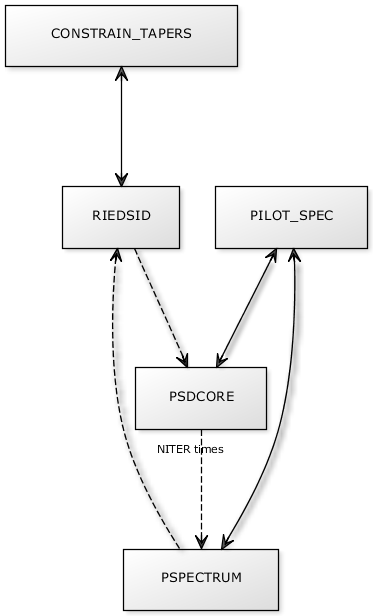
\includegraphics[width=0.5\textwidth]{yuml_d.png}%%
 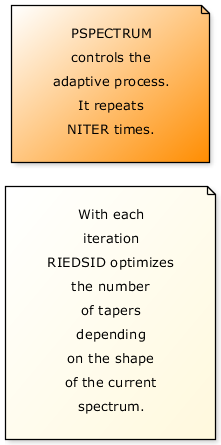
\includegraphics[width=0.3\textwidth]{yuml_n.png}
 \caption{Simplified call graph for \psd{}. The dashed lines show a
 simplified circuit
 which the spectra and its tapers make during the iterative process.}
 \label{fig:calls}
\end{figure}

\pagebreak
\section*{Session Info}
\begin{knitrout}
\definecolor{shadecolor}{rgb}{0.969, 0.969, 0.969}\color{fgcolor}\begin{kframe}
\begin{alltt}
\hlstd{utils}\hlopt{::}\hlkwd{sessionInfo}\hlstd{()}
\end{alltt}
\begin{verbatim}
## R version 3.1.2 (2014-10-31)
## Platform: x86_64-apple-darwin13.4.0 (64-bit)
## 
## locale:
## [1] en_US.UTF-8/en_US.UTF-8/en_US.UTF-8/C/en_US.UTF-8/en_US.UTF-8
## 
## attached base packages:
## [1] stats     graphics  grDevices utils     datasets  methods   base     
## 
## other attached packages:
## [1] bspec_1.4          ggplot2_1.0.0      signal_0.7-4      
## [4] RColorBrewer_1.1-2 RSEIS_3.3-3        psd_0.5-0         
## [7] fftw_1.0-3         knitr_1.9         
## 
## loaded via a namespace (and not attached):
##  [1] colorspace_1.2-4 digest_0.6.8     evaluate_0.5.5   formatR_1.0     
##  [5] grid_3.1.2       gtable_0.1.2     highr_0.4        lattice_0.20-29 
##  [9] MASS_7.3-37      munsell_0.4.2    plyr_1.8.1       proto_0.3-10    
## [13] Rcpp_0.11.4      reshape2_1.4.1   RPMG_2.1-5       Rwave_2.2       
## [17] scales_0.2.4     stringr_0.6.2    tools_3.1.2      zoo_1.7-11
\end{verbatim}
\end{kframe}
\end{knitrout}

%%
%\pagebreak
\bibliographystyle{apalike} %plainnat}
\bibliography{REFS}

\end{document}
